%!TEX root = ../dokumentation.tex


\chapter{Validierung des Systems}

Nachdem das Aufnehmen und Darstellen von Räumen funktioniert, wird die Genauigkeit des Systems untersucht. Zudem werden Versuche zu verschiedenen Auflösungen und unterschiedlicher Sensoren durchgeführt.  


\section{Genauigkeit des Systems}

Um die Genauigkeit des Systems zu überprüfen, wird ein Raum mit dem Lidar-System vermessen. Zudem wird der Raum händisch vermessen und der Grundriss mit der Software "Sweet Home 3D" erstellt. Anschließend wird die 3D-Darstellung mit dem Grundriss des Raumes und weiterer markanter Gegenstände verglichen.
Bei dem Raum handelt es sich um einen Flur mit vielen Ecken, Türen und Gegenständen. Dadurch erhält man viele verschiedene Maße, die überprüft werden können. Der Grundriss des Raumes ist in Bild ... dargestellt. Alle weiteren Maße des Raumes können direkt in der Software abgerufen werden.

\begin{figure}[H]
	\centering
	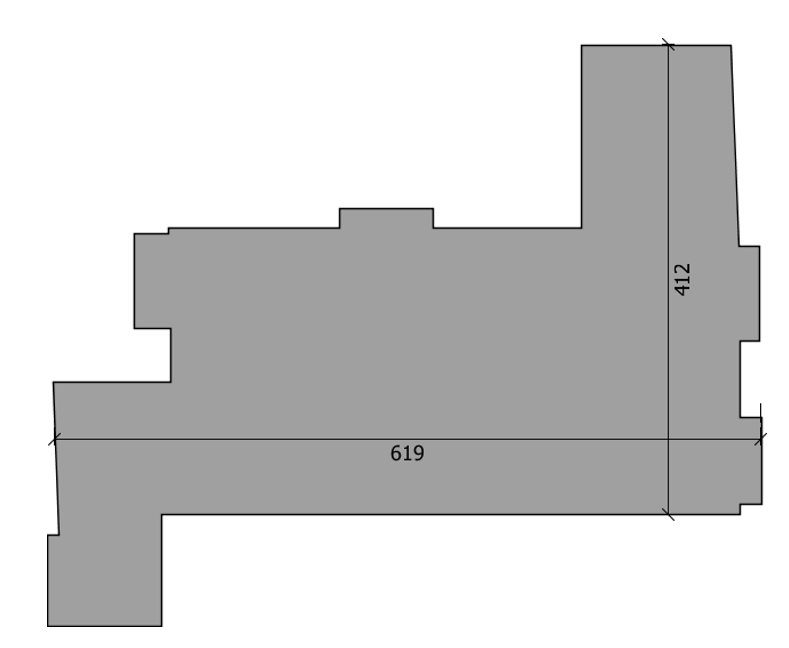
\includegraphics[width=0.7\textwidth]{images/Validierung/Grundriss}
	\caption{Grundriss des Testraums}
	\label{grundriss}
\end{figure}


Das Lidar-System wird im Raum aufgestellt, die Position ist annähernd mittig und wird zudem ausgemessen und in der Software eingetragen. Durch die Funktionsweise von Lidar Sensoren entstehen Schatten. So können beispielsweise Konturen hinter einer Wand, die die Lichtstraheln reflektiert nicht detektiert werden. Diese Schatten werden ebenfalls im Grundriss eingezeichnet, um den Vergleich besser durchführen zu können. Die weißen Stellen innerhalb des Grundrisses in Abbildung ... stellen diese Schatten dar.

\begin{figure}[H]
	\centering
	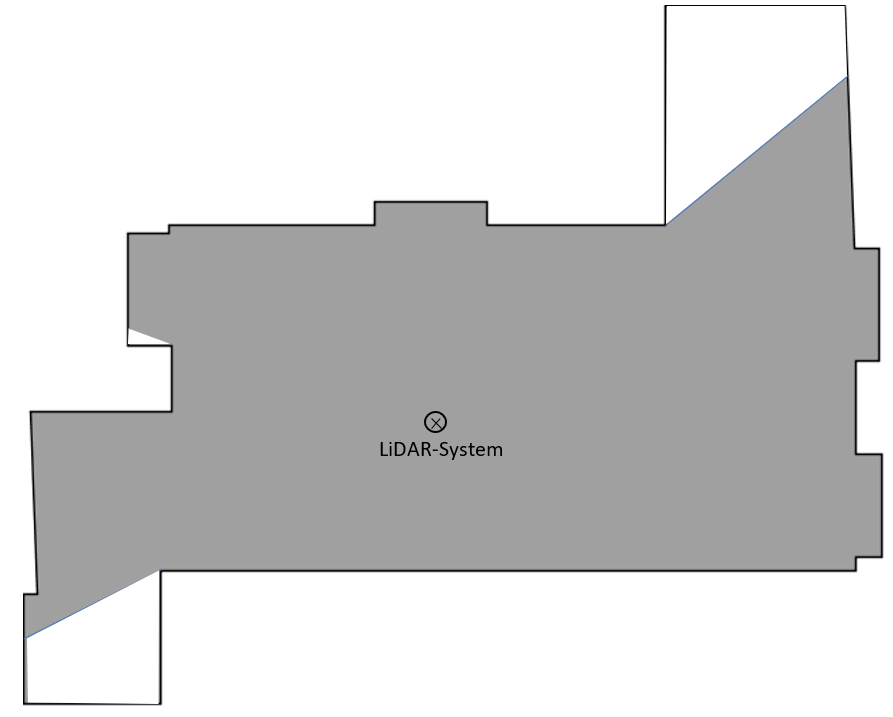
\includegraphics[width=0.7\textwidth]{images/Validierung/MitSchatten}
	\caption{Grundriss des Testraums}
	\label{grundrssmitschatte}
\end{figure}


Zum Vergleich wird nun der Grundriss benötigt, den das Lidar-System erstellt hat. Dazu wird die 3D Darstellung nur in z-Richtung betrachtet. Man erhält eine Vogelperpektive des Raumes, bei dem der Grundriss auszumachen ist. 

\begin{figure}[H]
	\centering
	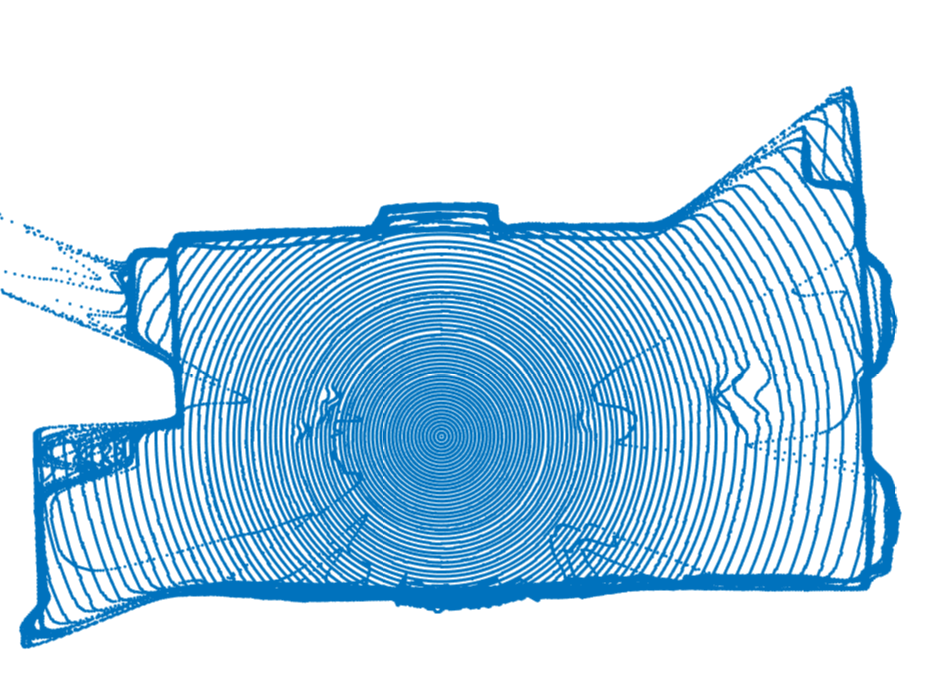
\includegraphics[width=0.7\textwidth]{images/Validierung/Vogelperspektive}
	\caption{Vogelperspektive des Testraums}
	\label{vogelperspektive}
\end{figure}


Zum grafischen Vergleich werden manuell erstellter Grundriss und die Vogelperspektive des Testraums mit einem Bildbearbeitungsprogramm im gleichen Maßstab übereinander gelegt.

\begin{figure}[H]
	\centering
	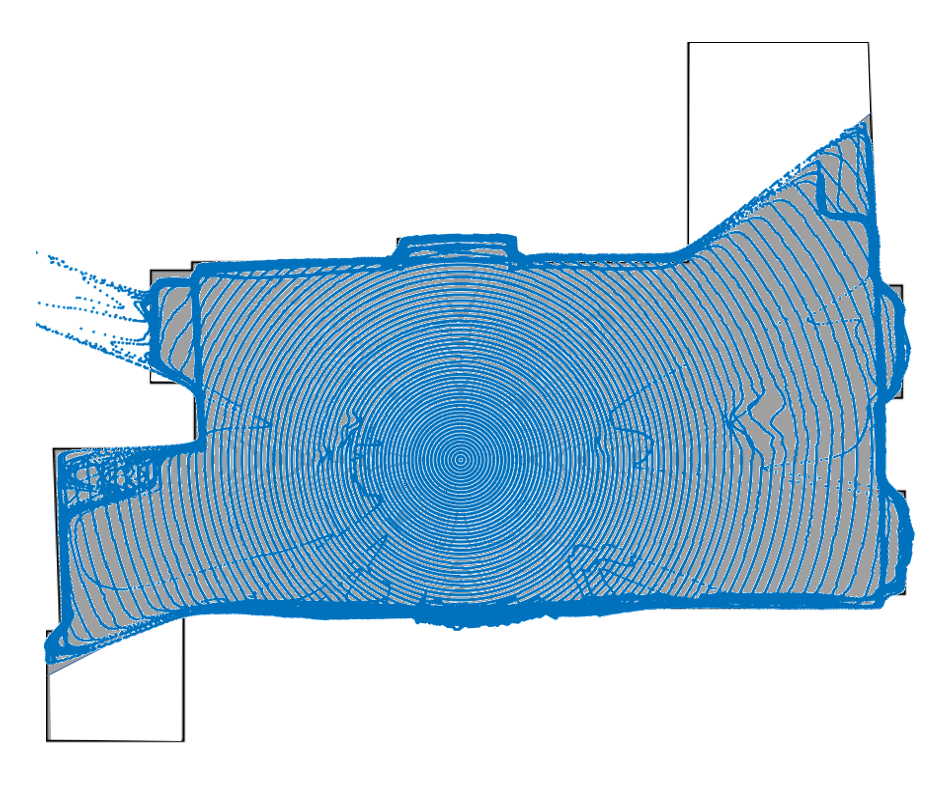
\includegraphics[width=0.7\textwidth]{images/Validierung/uebereinander}
	\caption{Grafischer Vergleich der Grundrisse}
	\label{uebereinander}
\end{figure}


-- Was kann man sehn?
--nur 2 Linien nehemn

-- Linien an Seite raus weil Glas

-- Höhe wird überprüft
Schrank, Bild usw

Messen mit Cursor



\section{Vergleich verschiedener Auflösungen}

Durch das Einstellen verschiedener Schrittweiten der Schrittmotoren können unterschiedliche Auflösungen und Punkteverteilungen eingestellt werden. Derselbe Raum wird unter den gleichen Randbedingungen mit drei unterschiedlichen Einstellungen vermessen. Dabei bleibt sowohl die Position des Lidar-Sensors als auch der Sensor selbst gleich. Verändert wird sowohl die horizontale Schrittweite als auch die vertikale Schrittweite. Dies kann im Code durch das Ändern weniger Parameter realisiert werden.

Bei den verschiedenen Auflösungen werden vor allem das Ergebnis und die benötigte Zeit zum Aufnehmen der Messdaten verglichen. Zudem soll dadurch eine Einstellung gefunden werden, die einen guten Kompromiss zwischen Auflösung und benötigter Zeit darstellt. 

Als Sensor wird immer der TF Mini Lidar verwendet.


\subsection{Übersicht über die Dauer, Auflösung und Anzahl an Messpunkten}

Die horizontale Auflösung wird im Code in achtel Schritten des Schrittmotors angegeben. Der Motor läuft im Achtelschrittbetrieb. Für eine gesamte Umdrehung des Motors werden 200 Vollschritte benötigt. Zudem entspricht die Übersetzung von Schrittmotor zur drehbaren Basis des Lidar-Systems 1:6. Es werden also 9600 Achtelschritte benötigt, um die Basis einmal um 360 Grad zu drehen. Die Auflösung in Grad bezogen auf die angabe im Code kann mit Formel... berechnet werden. 

\begin{equation}\formelentry{Berechnung horizontiale Auflösung}
d = \frac{360}{200 \cdot 8 \cdot 6} \cdot x
\end{equation}

Die vertikale Grundeinheit sind viertelschritte. Um den Sensor um die maximalen 90 Grad drehen zu können, werden 50 Vollschritte benötigt. Der Sensor ist direkt mit der Welle des Motors verbunden, wodurch keine Konstante für eine Übersetzung benötigt wird.

\begin{equation}\formelentry{Berechnung vertikale Auflösung}
d = \frac{360}{50 \cdot 4} \cdot x
\end{equation}


Die Anzahl der Messpunkte lässt sich über die Anzahl der horizontalen Messpunkte * Anzahl der vertikalen Reihen berechnen.



Die Berechnung der Zeit hängt 

\begin{center}
	\begin{tabular} [H] {|c|c|c|c|}
		\hline
		\textbf{}										 &\textbf{Auflösung gering} & \textbf{Auflösung mittel}	& \textbf{Auflösung hoch} \\ \hline
		\textbf{Auflösung horizontial [$^{\circ} $]}	 & 1,2 	& 0,15 	 & 0,15			\\ \hline
		\textbf{Auflösung vertikal [$ ^{\circ} $]}		 & 14,4 & 7,2 	 & 3,6  		\\ \hline
		\textbf{Anzahl Messpunkte}						 & 7524 & 120049 & 240099 		\\ \hline
		\textbf{Dauer [min]}							  	 & 4    & ?	 & ? 		 	\\ \hline
		
		\end {tabular}
		\captionof{table}{Übersicht verschiedene Auflösungen}
		\label{uebersicht}
	\end{center}


 


\subsection{Vergleich der Ergebnisse}


\begin{figure}[htb]
	\centering
	\begin{minipage}[t]{0.45\linewidth}
		\centering
		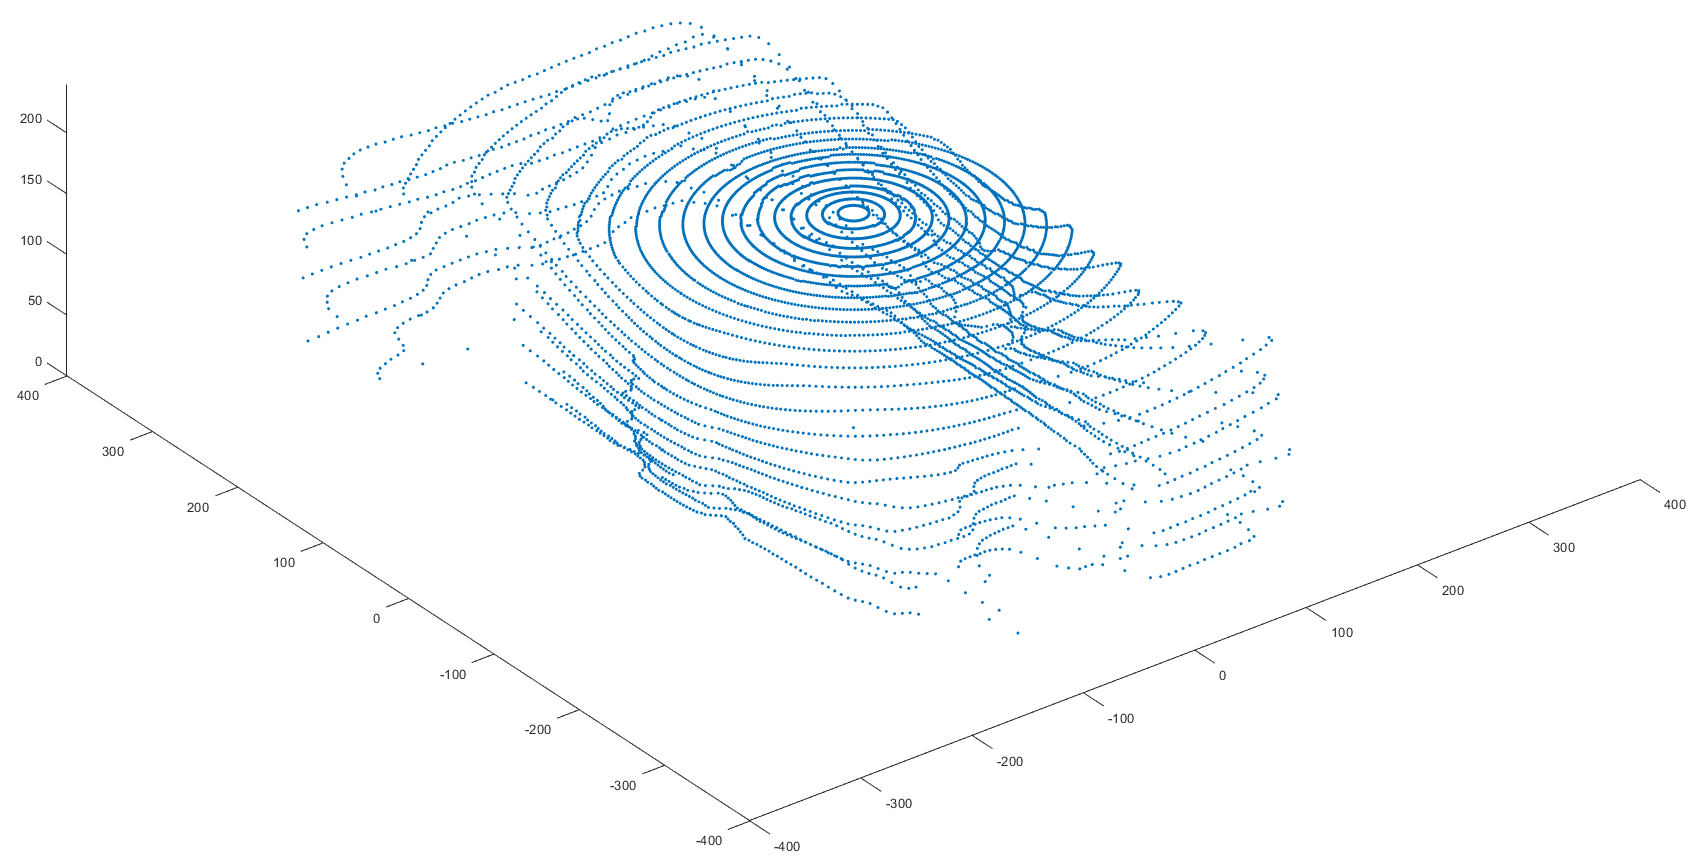
\includegraphics[width=1.2\linewidth]{images/Validierung/Aufloesungen/niedrig.png}
		\caption{Beispielbild}
	\end{minipage}
	\hfill
	\begin{minipage}[t]{0.45\linewidth}
		\centering
		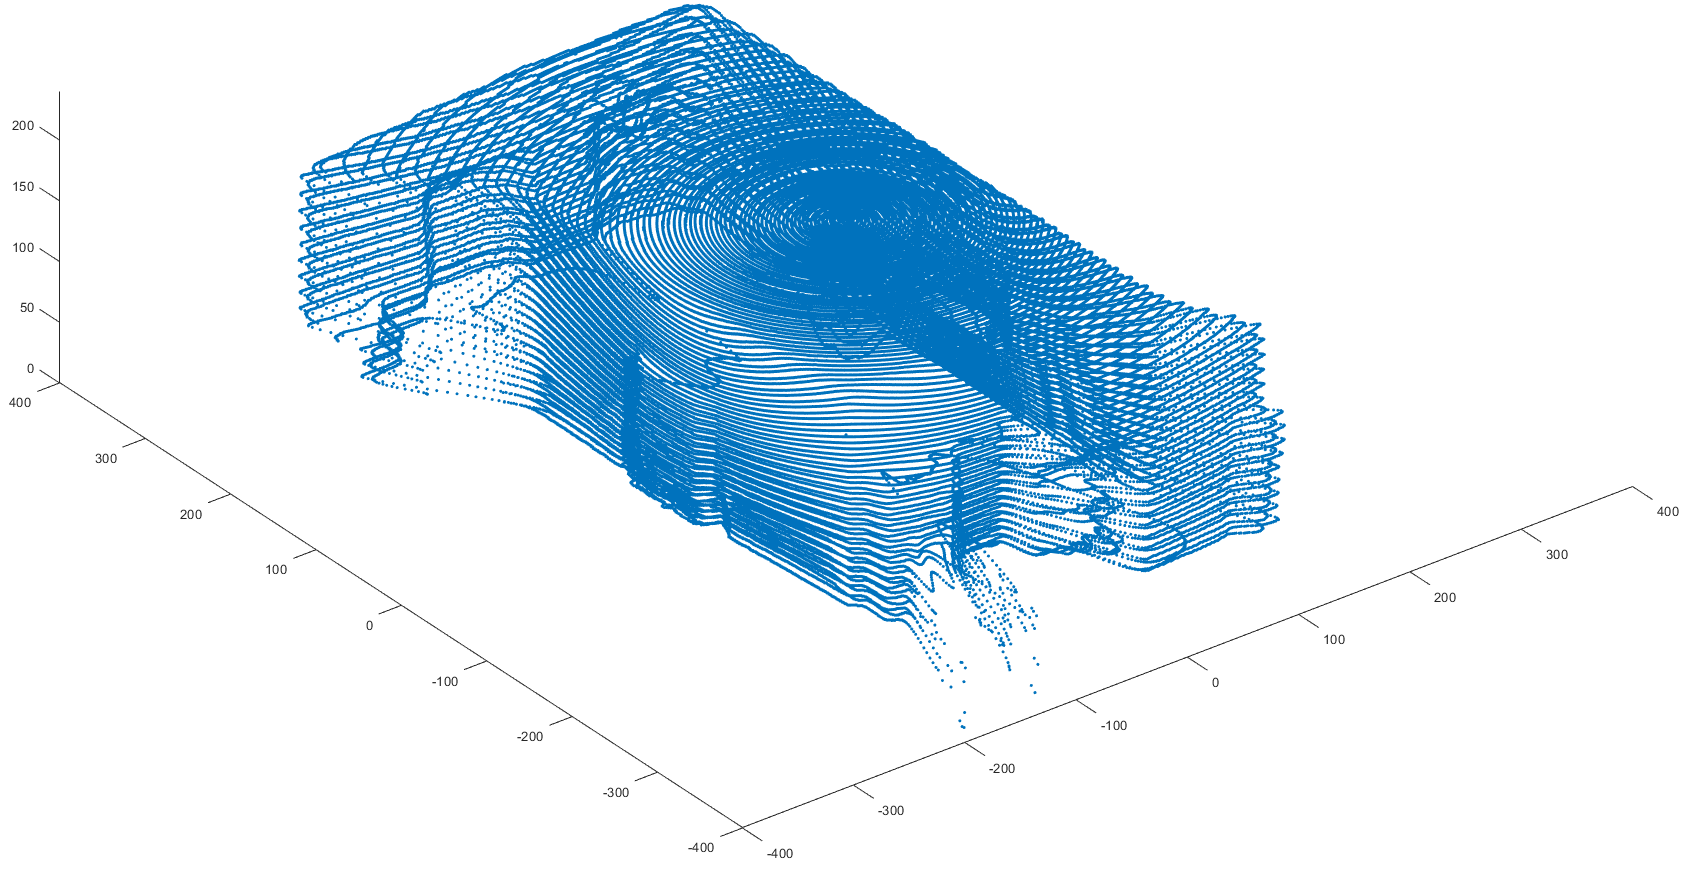
\includegraphics[width=1.2\linewidth]{images/Validierung/Aufloesungen/hoch.png}
		\caption{Beispielbild}
	\end{minipage}
\end{figure}






\section{Vergleich der Sensoren}